\documentclass[margin=2mm]{standalone}

\usepackage[
% school,
% simplified
]{pgf-umlcd}

%%%%%%%%%%%%%%%%%%%%%%%%%%%%%%%%%%%%%%%%%%%%%%%%%%%%%%%%%%%%%%%%%
\usepackage{listings}
\usepackage{color}
\definecolor{listinggray}{gray}{0.92}
\lstset{ %
language=[LaTeX]TeX,
breaklines=true,
frame=single,
% frameround=tttt,
basicstyle=\footnotesize\ttfamily,
backgroundcolor=\color{listinggray},
keywordstyle=\color{blue}
}
%%%%%%%%%%%%%%%%%%%%%%%%%%%%%%%%%%%%%%%%%%%%%%%%%%%%%%%%%%%%%%%%%

%%%%%%%%%%%%%%%%%%%%%%%%%%%%%%%%%%%%%%%%%%%%%%%%%%%%%%%%%%%%%%%%%
\usepackage{hyperref}
\hypersetup{
  colorlinks=true,
  linkcolor=blue,
  anchorcolor=black,
  citecolor=olive,
  filecolor=magenta,
  menucolor=red,
  urlcolor=blue
}
%%%%%%%%%%%%%%%%%%%%%%%%%%%%%%%%%%%%%%%%%%%%%%%%%%%%%%%%%%%%%%%%%

%\renewcommand{\umltextcolor}{red}
\renewcommand{\umlfillcolor}{black!6}
\renewcommand{\umldrawcolor}{red!60!black}

\newcommand{\selfcomposition}[4]
{
\draw[red!60!black,  -diamond] (#1) ++(#4, 0) -- ++(2cm,0) -- ++(0, -0.9cm) -- ++(-2cm,0)
node[near end, above]{#2}
node[near end, below]{#3};
}

\begin{document}

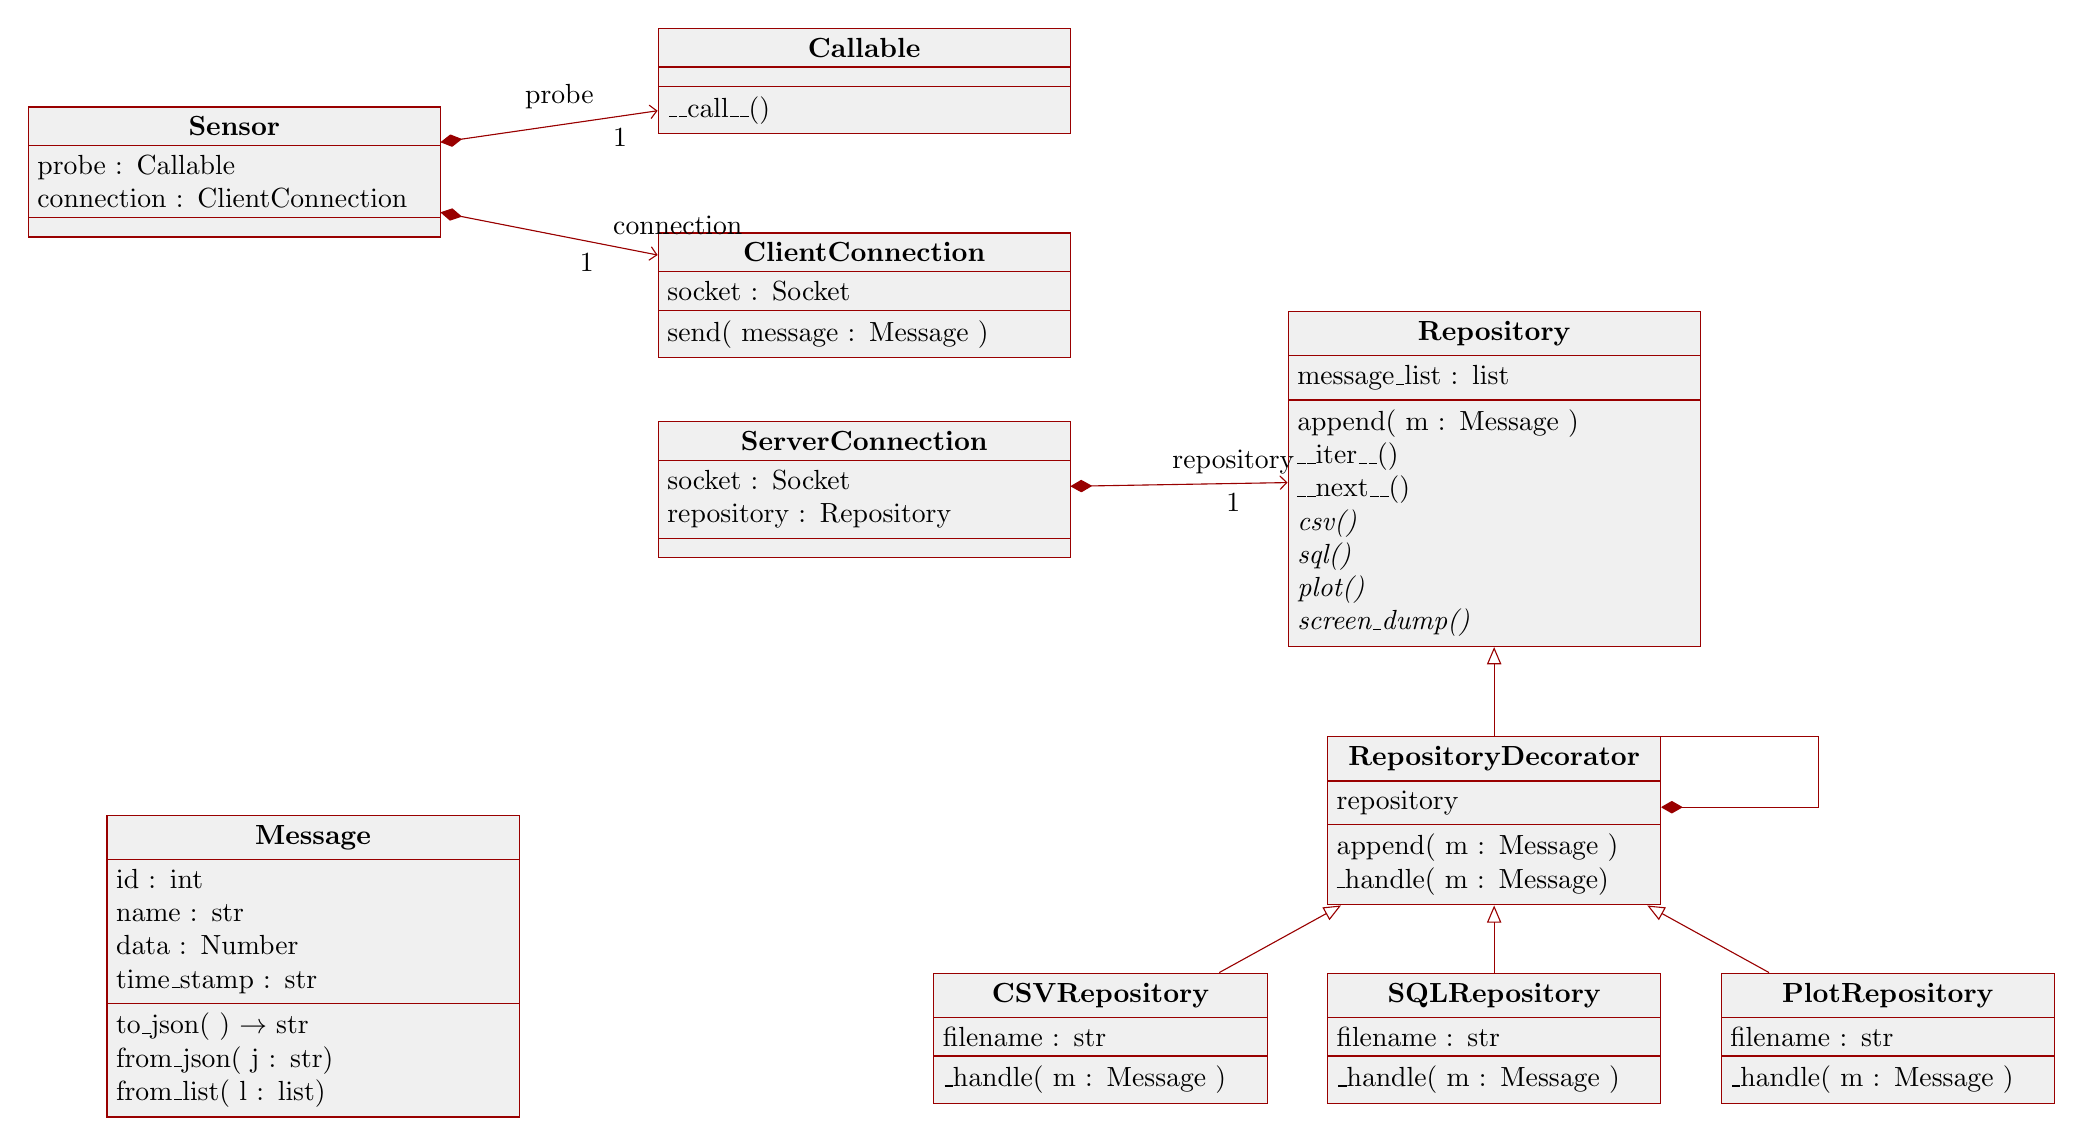
\begin{tikzpicture}[
  % show background grid
  ]
  \begin{class}{Sensor}{0,0}
    \attribute{probe : Callable}
    \attribute{connection : ClientConnection}
  \end{class}

  \begin{class}{Callable}{8, 1}
    \operation{\_\_call\_\_()}
  \end{class}

  \begin{class}{ClientConnection}{8,-1.6}
    \attribute{socket : Socket}
    \operation{send( message : Message )}
  \end{class}

  \composition{Sensor}{probe}{1}{Callable}
  \composition{Sensor}{connection}{1}{ClientConnection}


  \begin{class}{ServerConnection}{8,-4}
    \attribute{socket : Socket}
    \attribute{repository : Repository}
    
  \end{class}

  \begin{class}[text width = 5cm]{Repository}{16,-2.6}
    \attribute{message\_list : list}
    \operation{append( m : Message )}
    \operation{\_\_iter\_\_()}
    \operation{\_\_next\_\_()}
    \operation[0]{csv()}
    \operation[0]{sql()}
    \operation[0]{plot()}
    \operation[0]{screen\_dump()}
    
  \end{class}

  \composition{ServerConnection}{repository}{1}{Repository}


  \begin{class}[text width = 4cm]{RepositoryDecorator}{16,-8}
    \inherit{Repository}
    \attribute{repository}
    \operation{append( m : Message )}
    \operation{\_handle( m : Message)}
  \end{class}

  \selfcomposition{RepositoryDecorator.north east}{}{}{0cm}

  \begin{class}[text width=4cm]{CSVRepository}{11,-11}
    \inherit{RepositoryDecorator}
    \attribute{filename : str}
    \operation{\_handle( m : Message )}
  \end{class}

  
  \begin{class}[text width=4cm]{PlotRepository}{21,-11}
    \inherit{RepositoryDecorator}
    \attribute{filename : str}
    \operation{\_handle( m : Message )}
  \end{class}

    \begin{class}[text width=4cm]{SQLRepository}{16,-11}
      \inherit{RepositoryDecorator}
    \attribute{filename : str}
    \operation{\_handle( m : Message )}
  \end{class}


    \begin{class}[text width = 5cm]{Message}{1,-9}
      \attribute{id : int}
      \attribute{name : str}
      \attribute{data : Number}
      \attribute{time\_stamp : str}
      \operation{to\_json( ) \(\rightarrow\) str }
      \operation{from\_json( j : str) }
      \operation{from\_list( l : list) }
  \end{class}


\end{tikzpicture}
\end{document}
